\section{Methods}

\subsection{Architecture}\label{methods:Architecture}
    In Deep-Learning based compression, encoding comprises of the data first
    beeing transformed by a neural network into a latent space. Then this latent
    space is losslessly encoded and transmitted. On the decoding side, the
    latent space is decompressed and passed through another neural network back
    to the input domain.

    \begin{figure}
        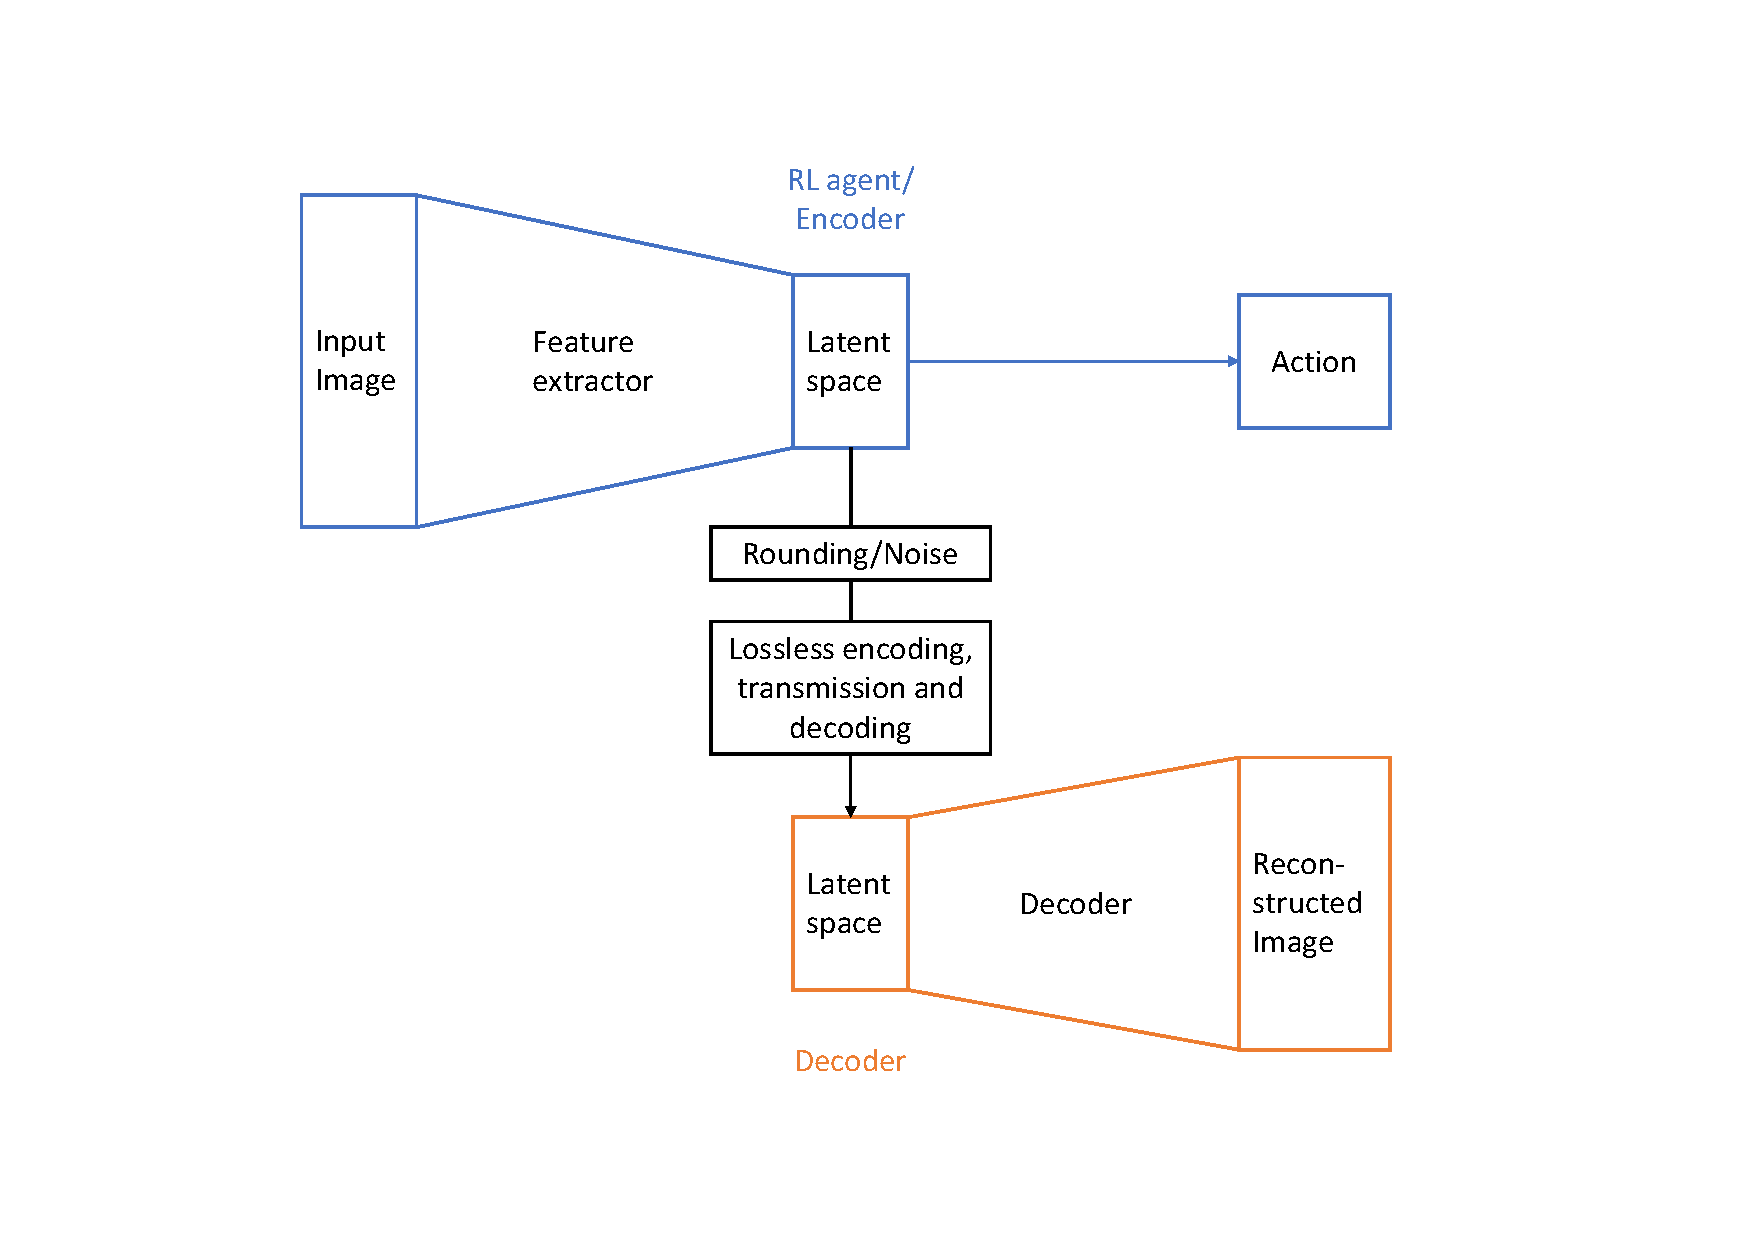
\includegraphics[width=\linewidth]{img/architecture.pdf}
        \caption{Overall architecture. First, the input image gets transformed by the feature extractor to the latent space. This latent space is used for the action of the agent as well as transmitted. The decoder then tries to reconstruct the input image from the latents.}
    \end{figure}

    In our approach, a Reinforcement Learning agent takes the place of the first
    neural network. The agent contains a so-called feature extractor, which
    extracts features from the observation that are important for determining
    the action. As described in ??, this information should also be important
    for reconstruction. Then the latent space is losslessly encoded and
    transmitted with an algorithm of choice (for example ..., for training this
    step is not strictly necessary as the latents get losslessly decompressed in
    the next step). After decoding the latents they are passed through the
    second network which in this case is a normal upsampling CNN (TODO: which name??). 

\subsection{Objective and evaluation in lossy compression}
    In traditional lossless image compression, the objective is to minimize the
    bitrate while still achieving a perfect reconstruction of the input data.
    Lossy compression on the other hand allows for distortions of the
    reconstruction, which leads to a tradeoff between distortion and bitrate. If
    the bitrate should be lower, one has to discard more information, leading to
    a worse reconstruction or higher distortion. Therefore the objective becomes
    to either to minimize the bitrate for a given distortion or minimize the
    distortion for a given bitrate.

    To determine the bitrate of an algorithm, one has to look at the encoding
    process of the data, see \ref{methods:Architecture}. The process should
    decrease the bitrate compared to the original input image, if the entropy of
    the latent space is lower than the input space, and a sufficiently fitting
    encoding distribution is chosen.

    If the distribution over the latent space is given by $Q_\theta(Z=z \vert x)$ where
    $\theta$ parametrizes the distribution and $P(Z=z)$ is used to encode the
    latents, the bitrate is given by the cross entropy
    \begin{equation}\label{eq:BitRate}
        \mathbb{E}_{z \sim Q_\theta(Z=z \vert x)}[log(P(Z=z))]
    \end{equation}
    As neural networks have real valued outputs so $Q_\theta(Z=z \vert x)$ is a
    continuous pdf, the bitrate is clearly very high. Therefore one approach is
    to round the latent values. This reduces $Q$ to a discrete probability
    distribution, which reduces the cross entropy. However, rounding is a
    undesirable operation during training, since the gradient is 0 nearly
    everywhere. Therefore, we replace the rounding during training by the
    addition of uniform noise, which shifts the values similarly to rounding,
    but is differentiable.
    
    Another effect is that we can reparametrize \ref{eq:BitRate} and take the
    expectation over the uniform noise:
    \begin{equation}
        \mathbb{E}_{u \sim U[-\epsilon, \epsilon]}[log(P(Z=\hat{z} + u))]
    \end{equation}
    where $\hat{z}$ is the mean of $Q_\theta(Z=z \vert x)$.

    % (To be more precise: We start with a continuous pdf. Rounding creates a
    % bunch of delta pulses which are nondifferentiable. However we can
    % approximate the continuous pdf by adding uniform noise to the new discrete
    % pdf. Therefore we can also just add noise instead of round?)

    
    % In turn, this means that the encoding network shouldn't encode information
    % in small differences. One approach to achieve this behaviours is to add
    % noise to the latent values, which forces the RL-agent to get more robust to
    % noise.

    % [TODO: this part is just disregared in balle]
    The encoding distribution $P$ is naively chosen to be a normal distibution. The
    mean can be chosen arbitrary given a powerful enough transformation, so is
    set to 0 for simplicity. The variance is also learned.


    Decreasing the bitrate is often traded against an increase in distortion.
    Therefore we need a performance measure to evaluate the distortion of the
    reconstructed image $\hat{x}$. A traditional metric is the Mean Squared Error (MSE),
    \begin{equation}
        \mathbb{E}_{x, \hat{x}}[\sum_{i,j} (x_{ij} - \hat{x_{ij}})^2]
    \end{equation}
    If humans look at images however, they often just care about specific types
    of distortion. A slightly lower brightness for example wouldn't matter for
    most images, but probably a different colour or more generally they care
    more about semantic distortion that would give them a different
    interpretation and representation of the image. MSE however gives these
    distoritions all the same values. Therefore, other distortion measures like
    MSSIM?? have been developed
    % TODO: write that part

    

    
    


% \subsection{Objective function from view of variational inference}
%     In Lossy image compression, the objective function is given by the ELBO:
%     \begin{align}
%         & \mathbb{E}_{z \sim Q(Z= z)}[log P(X, Z= z) - log Q(Z = z)]\\
%         & = \mathbb{E}_{z \sim Q(Z= z)}[log P(X \vert Z= z) - log \frac{Q(Z = z)}{P(Z = z)}]\\
%         & = \mathbb{E}_{z \sim Q(Z= z)}[log P(X \vert Z= z)] - D_{KL}[Q(Z = z)\Vert P(Z = z)]\\
%     \end{align}
    
%     Problem is, that we cannot differenciate by q since expectation is over q,
%     so just fix q by uniform distribution, and do reparametrization trick

%     now entropy of q becomes fixed so we can remove from optimization, just need
%     to care about $E_U[P(Z + U)]$

%     just need to choose encoding distribution, choose naively as normal with
%     mean 0 and learned variance since needs to be flexible.

%     for likelihood, choose normal (leads to MSE) and fix variance

\subsection{Training}
    RL-agents are normally trained with a specific loss function, which will be
    abstracted by $Loss_{RL}$. As the RL-agent takes the role of the encoder it
    is responsible for the bitrate. Therefore we add the loss from
    \ref{eq:BitRate} to the standard loss:
    \begin{equation}
        \mathbb{E}_{x}[Loss_{RL}(x) + \mathbb{E}_{u \sim U[-\epsilon, \epsilon]}[log(P(Z=\hat{z} + u))]]
    \end{equation}
    Both expectations will be approximated by empirical means over the training
    data. As the RL-agent is independent of the decoder, we can also train it
    separatly first.

    After training the RL-agent, we fix its values. Therefore at this point, the
    encoding to the latents is fixed. Now the decoder to the reconstruction
    needs to be trained. For the decoder, we use the loss given in TODO: add ref. 

\subsection{Decoder loss}
For our decoder, we tried several loss functions. The simplest version was the MSE between the original and reconstructed images. \\
In early experimentation (see section 4.1), we found that some details which may be considered important to the task, specifically the location of the ball, were omitted as they accumulated little MSE penalty; in an attempt to recover these aspects, we devised a second loss scheme, which we refer to as latent loss. The motivation was to reward the decoder for reconstructing the image in such a way that the same features would be extracted, resulting in preserving the most important aspects. For this loss, we passed the reconstructed image through the feature extractor and evaluated the MSE between the original latent space and the reconstructed latent space.










structure:
1. describe general architecture
2. describe goals and objective functions during training
3. training process